% -----------
% SETUP
% -----------
\documentclass{physics_article_B}
\title{Mechanical Vibrations of Droplets in Fluidic Systems}
\mytitle{Mechanical Vibrations of Droplets in Fluidic Systems}
\myname{Dominic Coy \& Oliver Gordon}
\studentid{4227789 \& 4224942}
\date{Due Date: 1 June 2018}

\begin{document}
	
% ----------------------
% COVERSHEET
% ----------------------
\pagenumbering{roman} 
\setcounter{page}{0}
%\includepdf[scale=1]{Images/Cover.pdf}
%\maketitle

% ----------------------
% ABSTRACT
% ----------------------
\pagenumbering{gobble} 
\begin{abstract}
	\large{Stuff
}
\end{abstract}
	
% ----------------------
% CONTENTS
% ----------------------
%\vspace{4cm}

\tableofcontents

\pagenumbering{roman} 
\setcounter{page}{1}
	
% ----------------------
% INTRODUCTION
% ----------------------
\newpage
\pagenumbering{arabic} 
\setcounter{page}{1}

% ----------------------
% Literature Review
% ----------------------

\section{Combined Intro\label{sect:theory1}}

Simultaneously measuring the viscosity and surface tension of fluids has, in the past, been challenging especially with small volumes of fluid\textsuperscript{\cite{harrold}}. The most promising method involves vibrating small droplets\textsuperscript{\cite{harrold}} which only requires a few milliliters of liquid. This makes analysing rare or expensive liquids more viable than other conventional methods such as drop volume or microrheology\textsuperscript{\cite{harrold2}}. For a Newtonian liquid, frequencies and spectral widths of oscillation are well known, and these can be used to determine its physical properties. However, there is not much data for isolated viscoelastic droplets\textsuperscript{\cite{temperton}}. Our experiment aims to build a high-throughput system to measure the properties of many droplets. It is also known that impurities in single droplets, such as particles or polymers, can affect their rheological and surface properties\textsuperscript{\cite{temperton}}. This influences physical properties of the droplets such as the spreading, wetting and dewetting\textsuperscript{\cite{bergeron}}. This alteration can also affect their performance in various applications including fuel injection\textsuperscript{\cite{vukasinovic}}, inkjet printing and microscale mixing/demixing\textsuperscript{\cite{mugele}}. Research suggests that the viscoelastic vibrational modes of droplets may affect many areas of physics including crustal deformation of planets\textsuperscript{\cite{pollitz}}, dynamical properties of atomic nuclei\textsuperscript{\cite{wong}} and energy relaxation mechanisms in neutron stars\textsuperscript{\cite{bastrukov}}. 

There are multiple advantages of using vibrational spectra to determine rheological properties when compared to conventional methods such as drop volume and microrheology. For one, only a small amount of fluid on the order of mL\cite{temperton2014mechanical} is required. This makes it viable to investigate expensive and rare materials. Properties can also be tracked in real time, as demonstrated by Harrold et al. in 2016\cite{harrold2016optovibrometry} before their droplets became contaminated by airborne particles. This could be applied to lab-on-a-chip systems, allowing chemical reactions to be tracked live. There is therefore a significant impetus to investigate droplets containing mixed fluids, despite little work done to this end outside of this 2016 paper. Other applications of this vibrational method and supporting theory include monitoring inkjet printing performance\cite{martin2008inkjet}, simulating the crustal deformation of planets\cite{background}, and studying energy relaxation in stars\cite{background}.\\

The measurement of the physical properties of small droplets submerged within another fluid using vibrational techniques could, in the future, allow us to find the viscosity of either the droplets or the fluid surrounding them\textsuperscript{\cite{backholm}}. Alternatively, we could find the interfacial tension between the two liquids\textsuperscript{\cite{backholm}}. Our experiment aims to build a high-throughput system which could analyse many droplet's physical properties. This system could be extended to perform simultaneous measurements allowing research into how the viscosity and interfacial tension of fluids change during a chemical reaction\textsuperscript{\cite{backholm}}. As this experiment has relevance in microfluidics, future research could investigate lab-on-a-chip based applications\textsuperscript{\cite{tempertonphd}} such as an inexpensive, accurate and reliable diagnostic device\textsuperscript{\cite{yager}} for medical diagnosis in developing countries.

Many recent experiments have analysed levitated droplets using methods including magnetic\textsuperscript{\cite{hill}}, electrostatic\textsuperscript{\cite{mugele}}, acoustic\textsuperscript{\cite{trinh}}, aerodynamic\textsuperscript{\cite{benmore}} and fluidic\textsuperscript{\cite{backholm}}. Even though Backholm et al. studied sessile droplets (lying on a surface) within a fluid\textsuperscript{\cite{backholm}}, there seems to have been limited work done on fluidically levitated droplets. Both sessile droplets and pendant droplets (hanging off an object) are easier to produce than levitated droplets but incur additional energy dissipation mechanisms from the proximity of a surface to the droplet. This affects the damping coefficients of the droplets which changes their vibrational spectra  affecting results\textsuperscript{\cite{sharp}}. These mechanisms can be avoided using either superhydrophobic or superamphiphobic surfaces as the droplets take on a spherical shape and can be described with similar equations to levitated droplets. McHale et al. demonstrated the feasibility of this method using vibrating liquid marbles (droplets stabilised by the adsorption of small particles). However, they found that the particles dominated the droplet's physical properties and so the application of this approach is limited\textsuperscript{\cite{mchale}}.  Harrold et al. also showed that the analysis of vibrational frequencies can be used to track the material properties of droplets over time\textsuperscript{\cite{harrold2}}. Their results agreed with prior work until their droplets became contaminated with airborne particles\textsuperscript{\cite{harrold2}}. However, they showed that this technique could be adapted to study time-dependent, soft matter systems.

\section{Combined Lit Review\label{sect:theory}}

\subsection{History}
It has been known for some time that the vibrational spectra of small droplets can be exploited to determine various material properties. Building on the work\cite{rayleigh1879capillary} of Rayleigh in 1879, Chandrasekhar and Velentine in 1959\cite{chandrasekhar1959oscillations} and 1965\cite{velentine1965motion}, respectively, developed theoretical models relating the damping coefficients and oscillation frequencies of simple Newtonian liquids (such as water) to their viscosities. Multiple authors confirmed this experimentally in the 1990s\cite{egry1998viscosity,meier2000surface}. \\

Building on the work by Rayleigh in 1879, which related the frequency of oscillation of fluidic jets with their area and pressure\textsuperscript{\cite{rayleigh}}, in 1932 Lamb et al. derived an expression for the oscillation frequency of inviscid droplets in an inviscid fluid. They also derived approximate expressions for the rate of damping of oscillations in a viscous droplet in an inviscid fluid and for the oscillations of a bubble of gas in a low viscosity liquid. \\

In their derivations, the velocity fields found for small oscillations of an inviscid fluid were used to estimate the rate of viscous dissipation (rate that shear forces turn work done by a fluid on adjacent layers into heat) in a droplet with small viscosity\textsuperscript{\cite{lamb}}. Then, in 1960, Reid analysed the oscillations of a viscous droplet in a low-density gas or a vacuum\textsuperscript{\cite{reid}}. His experiment and analysis were summarised in the book Hydrodynamics and Hydrodynamic Stability by Chandrasekhar in 1961\textsuperscript{\cite{chandrasekhar}}. In 1965, Velentine et al. used the same methods as Lamb et al. to derive expressions for the damping rate of oscillations when a low viscosity droplet was submerged in a low viscosity fluid\textsuperscript{\cite{velentine}}. In 1968, Miller et al. derived a general dispersion equation for the oscillations of viscous droplets immersed in a viscous fluid, which could also be applied when the interface between the two fluids possessed elastic and viscous properties of its own. They also derived equations for the  rate of damping of oscillations and frequency for specific cases including when the interface between the two fluids is free or is inextensible\textsuperscript{\cite{miller}}.\\

Early experiments using droplets were based on theoretical models developed by Rayleigh\textsuperscript{\cite{rayleigh}} and Chandrasekhar\textsuperscript{\cite{chandrasekhar2}} who showed that, by using simple equations, vibrational frequencies of droplets were related to the viscosity and surface tension of a free liquid globe (essentially a levitated droplet). Much of the initial research within this area looks to have been driven by the ambition to study containerless crystallisation of pure liquids in microgravity\textsuperscript{\cite{wilkes}}. However, this approach was later adapted by multiple authors who demonstrated that analysing droplet vibrations could be used to extract frequency dependent physical properties of viscoelastic droplets\textsuperscript{\cite{egry}}. Temperton et al. claim to be the first to present a combined theoretical and experimental study in 2014\textsuperscript{\cite{temperton}}.

Although research was initially based around studying the crystallisation of pure liquids in microgravity\cite{Wilkes1997}, later authors such as Temperton expanded upon these simple models to derive other equations linking the vibrational spectra of a droplet to its rheological properties such as viscosity, $\eta$, surface tension, $\gamma$, and frequency dependant storage and loss moduli, $G'$ and $G''$. \\

\subsection{Other Droplet Shapes}

Over the years, experiments have focused on a variety of droplet shapes. Two of the three common droplet geometries are sessile (suspended on a surface)\cite{thesis, background, backholm2017oscillating} and pendant (teardrop-shaped and suspended off a surface such as a needle)\cite{thesis}. Despite the relative experimental ease of investigating these suspended droplets, damping interactions and droplet shape can be influenced by the suspension surface or the pipette used to transport them\cite{sharpscaling}. This alters the vibrational spectra, producing errors yet to be fully rectified\cite{harrold2016rheological}. Despite this, many authors limit such experiments to a single surface\cite{sharpscaling}, leading to differing results. Although McHale et al. demonstrated that the shape of the droplet can be somewhat controlled for by using superhydrophobic and superamphiphobic substances, this is not always practical as the rheological properties of the droplet are affected by these substances.

One of the main advantages of fluidic levitation involves lower mass loss. During an experiment, mass will be lost as the droplet evaporates over time. For fluidic levitation, this has been shown to be 2-4\%, which is significantly lower than for other methods which see over 10\% \cite{harrold2016optovibrometry} mass loss. However, to the best of our knowledge no author has modelled this mass loss and taken it into account. Furthermore, the way in which mass is calculated is also very basic; the droplet is weighed before and after an experiment by comparing the mass of a syringe or paper towel both with and without the droplet. These methods do not take into account leftover residue, and in the case of paper towels are destructive. Additionally, this method of levitation requires placing droplets by hand, which is a slow process. There is therefore a significant impetus to develop a high throughput system allowing multiple droplets to be quickly analysed in a hands-off fashion.\\

Although a great deal of research has been performed into determining the rheological properties of simple Newtonian liquids, the oscillations of isolated viscoelastic fluids (such as polymer solutions) have not been as thoroughly investigated; Temperton et al. claimed to be the first to present a combined theoretical and experimental study in 2014\cite{temperton2014mechanical}. However, their calculations relied on knowledge of $\gamma$, making a complete analysis yet to be achieved. To the best of our knowledge, viscoelastic droplets are yet to be analysed in this fashion.

As such, we intend to investigate the other common droplet shape of spherical droplets. These are formed by levitating fluid away from a surface using methods such as magnetic\cite{temperton2014mechanical, levitate2}, electrostatic\cite{mugele2006microfluidic, wong1981dynamics}, aerodynamic\cite{benmore2017aerodynamic}, acoustic\cite{thesis, yarin1998acoustic}, and fluidic levitation. Fluidic levitation is achieved by placing a droplet of fluid within a suspension medium of different viscosity. Besides spherical droplets, sessile droplets can also be investigated in this fashion by placing them on a suspension slide, as recently demonstrated by Backholm et al\cite{backholm2017oscillating}. These authors also showed that\cite{backholm2017oscillating} by using fluidic levitation, it is possible to determine both the interfacial tension between the droplet and the surrounding liquid, and the rheological properties of the surrounding liquid.\\

As the capillary length may not always be known, it is imperative that droplets are kept as small as possible as of Equation 1. However, it is possible to investigate larger spherical droplets by performing the experiment in low gravity; this was done in 1979\cite{holt1997surface} on Space Shuttle Columbia and resulted in similar findings to the other experiments discussed here. However, this is obviously impractical for our purposes.\\

\subsection{Computer Vision}

\section{Theory\label{sect:theory}}

    Following on from prior work, we will be making the major assumption that our droplets will be perfectly spherical. Below the capillary length of the material $l_{cap}$, surface tension, $\gamma$, dominates over gravitational interactions, $g_{eff}$. This results in the lowest energy configuration of the droplet to be spherical. As such, it is important that any droplet investigated has radius, $R$, lower than its capillary length. \\
    
    Because the droplet has an equilibrium spherical shape, it will undergo shape oscillations when a small perturbation is applied\cite{oscillation}. If this pertubation is in the from of an impulse, the surface of the droplet vibrates at its resonant frequency. This occurs as an impulse drives the surface of the droplet at all frequencies (owing to the mathematics of Fourier transforming a delta function). Vibrations not equal to the resonant frequency are damped, leaving only the vibrations at the resonant frequency of the droplet with a non-zero amplitude. For optimal results, it has been shown that any applied impulse must be long enough to give sufficient time to perturb the drop, but short enough to still be an impulse and not drive the droplet at a particular frequency\cite{temperton2014mechanical}. Furthermore, the amplitude of oscillations must be kept to under 0.1$R$, following work from Becker et al. who found that above this limit oscillations become non-linear, causing the simple equations used here to fail\cite{becker1991experimental}.\\
    
    These oscillations can be readily observed by placing a water droplet on a hydrophobic plate and gently blowing on it. A laser and photodiode (discussed further in Section X) can be used to detect this, giving a time dependant signal such as the one shown in Figure X. The frequencies that remain correspond to different modes, $n$, of oscillation. The $n=1$ node corresponds to oscillations of the droplet's centre of mass\textsuperscript{\cite{miller}}, whilst the $n\geq2$ nodes correspond to the surface oscillations which are of interest here. The corresponding frequency, $f_n$, and full-width-half-maxima, $\Delta f_n$, can then be calculated by fourier transforming the oscillatory signal. An example signal is shown in Figure Y. \\
    
    From here, it is possible to calculate the surface tension, $\gamma$, and viscosity, $\eta$, of the fluid using the equations
 
    \begin{equation} 
    \label{eq:SurfaceTension}
    \gamma = \frac{4\rho R^{2}}{\pi n^{2}}(\Delta f^{2} + f^{2}),
    \end{equation}
    
    \begin{equation} 
    \label{eq:Viscosity}
    \eta = \frac{\pi \rho \Delta f R^{2}}{n^{2}},
    \end{equation}

    where $\rho$ is the density of the droplet. To determine $R$, checkerboards of known dimensions can be used to map the pixels on a screen to real world space. Because cameras have no depth-perception, this requires the assumption that the object of interest is in the same plane as the checkerboard. Once the height and width of a spherical droplet, $R_x$ and $R_y$ respectively, has been found in an image containing a checkerboard, $R$ can be calculated with simple trigonometry:
            
            \begin{equation}\label{eq:radii}
                r = \sqrt{\Big(\frac{R_x}{2}\Big)^2 + \Big(\frac{R_y}{2}\Big)^2} .
            \end{equation}
    
    However, Equations \ref{eq:SurfaceTension} and \ref{eq:Viscosity} are only valid for simple Newtonian droplets such as water and glyercol. For viscoelastic droplets such as... , there is to date yet to be a complete analysis of droplets without prior knowledge of $\gamma$.
% ----------------------
% Equipment
% ----------------------
\section{Methods\label{sect:loop}}

    \subsection{Slide \& Fluid Loop}
    
        To interrogate liquids of interest, a clean test environment had to be created. This was accomplished by first creating a plastic mould with a 2 mm diameter tunnel inside. This tunnel size was large enough to allow...  The mould was then filled with PDMS, placed on a glass slide and cured. A 1 mm port was also created on the top side of the slide, and subsequently used to inject fluids of interest. This smaller diameter was chosen as the higher pressure it created prevented backflow/droplets constantly flowing when only a single droplet was ever desired in the slide at any one time.\\
        
        Three capillary tubes were then attached these ports, before sealing all leaks with flowable silicon. This setup is demonstrated in Figure \ref{fig:control}. Because of the difficulties and long drying times involved with manufacturing perfectly sealed PDMS slides with smooth tunnels, we later changed to perspex instead of glass/PDMS, and carefully drilling the appropriate holes. This had the advantage of being quicker to produce, less fragile, and less prone to internal leaking. \\
        
            \begin{figure}[H]
            \centering
            \hspace*{2cm}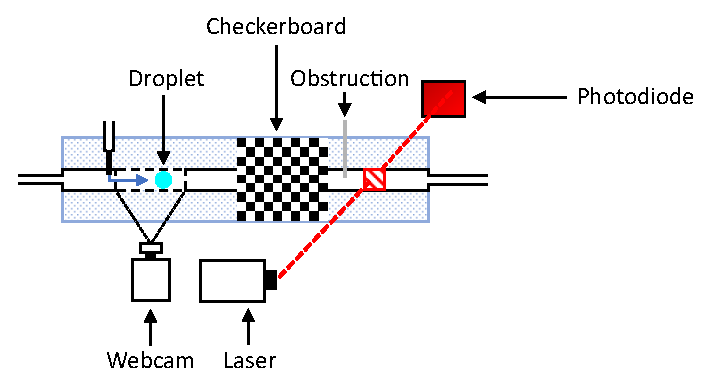
\includegraphics[scale=0.9]{Figures/Control.eps}
            \captionsetup{justification=centering}
            \caption{Words.} 	
            \label{fig:control}
            \end{figure} 
    
        To move droplets through the slide, the capillary tubes were then connected to a fluid loop consisting of 3 mm (?) tubes. To transport the spherical droplets, mineral oil of a lower viscosity was used as a carrier medium. A microfluidics motor was used to transport the oil from a central reservoir and around the loop. To reduce stress on the capillary tubes of the slide, the motor was attached on the "in" side, so oil is not being pulled against the external tubes, potentially breaking them (?). A t-junction was also placed at the return side of the loop to allow for easy bleeding of air. After being interrogated in the slide, droplets were transported to the reservoir. Here, they could be easily removed by hand, as the droplets were of different density to the mineral oil, so would either sink or float. To prevent these droplets from returning into the flow system, the return and collection tubes were placed at different heights on opposite sides of the reservoir. This setup is demonstrated in Figure \ref{fig:basic}.
        
            \begin{figure}[H]
            \centering
            \hspace*{2.0cm}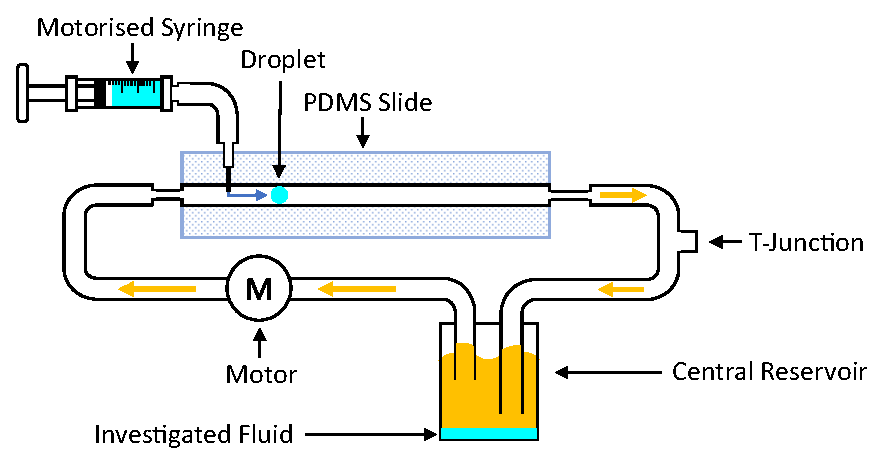
\includegraphics[scale=0.8]{Figures/Fluid.eps}
            \captionsetup{justification=centering}
            \caption{Words.} 	
            \label{fig:basic}
            \end{figure} 

    \subsection{Motor \& Syringe Pump}

        To allow the speed of the fluid to programmatically controlled as part of the computer vision system described below, the motor had to be driven by a DAQ card. However, the card used lacked the circuitry to output sufficient current, making it unable to turn the motor at any voltage. Furthermore, the card had poor output resolution, making very fine control of fluid speed impossible. A current boosting circuit was therefore produced, and is shown in Figure \ref{fig:MotorCircuit}. Besides using an external power supply to increase output current to suitable levels, it maps the 0-4 V input rating of the motor to the full 0-10 V output of the DAQ, effectively increasing its sensitivity. Resistances were chosen both to provide the required output and provide good heat dissipation. Heat dissipation was further improved by attaching a heatsink to the transistor. The 12 $\Omega$ resistor was also replaced with 3 x 36 $\Omega$ resistors to reduce component stress. The motor was given protection by powering the circuit with a current limited power supply set at the maximum current rating of the motor. 
        
            \begin{figure}[H]
                \centering
                \hspace*{-1.8cm}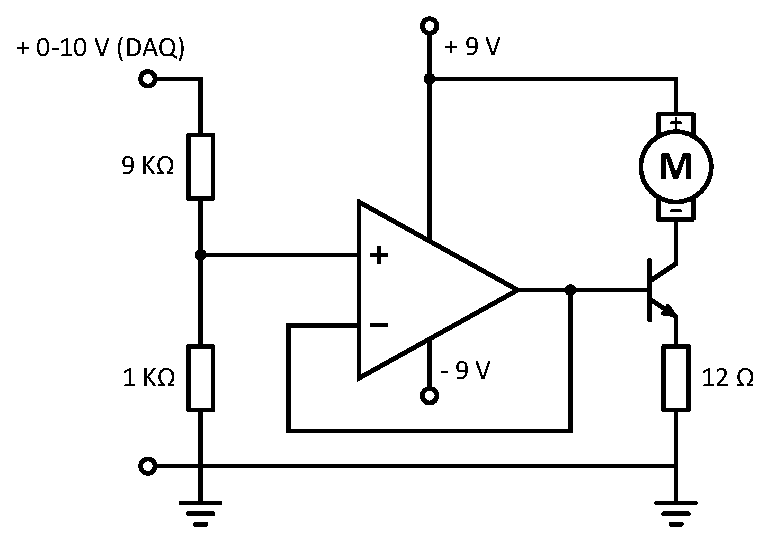
\includegraphics[scale=0.8]{Figures/MotorCircuit.eps}
                \caption{Caption}
                \label{fig:MotorCircuit}
            \end{figure}
        
        To allow droplets of a consistent size of be created, a motorised syringe pump was set up, and code created to automatically interface over a COM port. To decrease the size of droplets being produced, the speed of the motor could be increased. However, droplets needed to be moved as slowly as possible to increase the time of data collection. Droplet size could therefore be made larger by increasing the speed at which the syringe pump was turned by writing code to interface with the pump through a serial port. A large syringe (name?) was chosen.
        
        
    \subsection{Determining Density}
    
        For more manual experimentation, $\rho$ is calculated by determining $R$ of a spherical droplet (and therefore its volume). The mass is then measured by absorbing a droplet onto a paper towel and comparing to the mass without the droplet\cite{hill}. This method is both destructive and erroneous by up to 10\%\cite{harrold2016optovibrometry} due to mass loss during the experiment. It is also not viable for our purposes, as our droplets are suspended in fluid. 
        By holding our fluid of interest in a syringe, we instead determine mass by comparing the mass of an empty and filled syringe. The volume can be easily determined by reading from the scale of the syringe.\\
    
        This method has multiple advantages. For one, the method is non-destructive, making it more practical for many biological investigations such as protein crystallisation  studies\textsuperscript{\cite{zhu}} and cell culture bioreactors\textsuperscript{\cite{konry}}, or any time where an expensive/rare liquid needs to be recovered\cite{backholm}. Further, as the system is self contained and has all measurements taken within seconds, no mass can be lost to evaporation during the experiment. This has been shown to introduce errors to density as high as 10\%. Further, averaging down from larger volumes results in a lower percentage error per droplet, improving accuracy.
        
    \subsection{Computer Vision\label{sect_vision}}
        
        \subsubsection{Acquiring Data}
            In order to allow droplets to be analysed in real time, a computer vision control system was developed. A Logitech C920 camera was chosen for its high image quality, high resolution, and wide field of view. \\
            
            Because droplets are not static, strict requirements are placed on the efficiency of calculations. Furthermore, as MATLAB is an interpreted language and lacks hardware acceleration, webcam acquisition operates at very low framerates, making tracking moving droplets in real time difficult. This was overcome by modifying Hebicam\cite{HebiCam}, which was originally created for streaming CCTV footage, and is a MATLAB wrapper for the more efficient openCV. After adapting this package for use with USB webcams, 1080p video could be acquired at 30FPS with spare processor overhead to perform calculations, as opposed to 6 with none. Furthermore, data was acquired in grayscale (as opposed to RGB), further increasing capture efficiency and reducing the size of stored data. 
            
    
        \subsubsection{Calibration}

            To ensure that droplets were calculated accurately, we applied checkerboard calibration. 20 images of a 10 x 11, 0.20 mm checkerboard pattern were taken at different positions in similar positions to those used during our experiment. The positions of the checkerboard in the calibration screenshots as determined by the algorithm are shown in Figure \ref{fig:calib}. An algorithm implemented in MATLAB\cite{CameraCalibration} was then used to calculate various extrinsic properties of the camera, such as the optical centre, distortions, and focal lengths in x and y. 
            
                \begin{figure}[H]
                    \centering       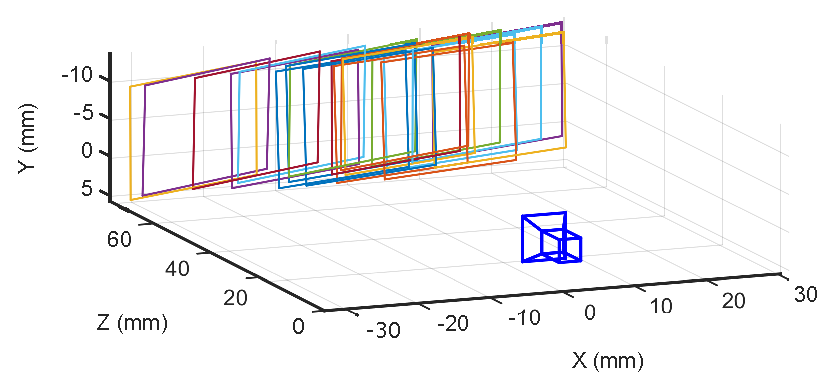
\includegraphics{Figures/CameraExtrinsics.eps}
                    \caption{Figure }\label{fig:calib}
                \end{figure}
        
            To calculate the size of an object and because a webcam has no depth perception, the checkerboard had to be placed in plane with the droplets. Because the slide was of a finite size, a limitation was placed on the size of the checkerboard. Larger checkers had a lower percentage error from imperfect focusing, yet less of them could be placed on a slide. \\
            
            There was an added complication to this process in that the PDMA used to create the experiment area was not perfectly flat. Because the algorithms work on the assumptions that checkerboard is flat and the droplet is in plane with the checkerboard, the pattern was instead printed on a long piece of paper, carefully folded and tensioned to the back of the slide. However, this resulted in a small 1mm disparity in depth between the droplet and the checkerboard, resulting in a small error. Using simple trigonometry to measure the distance to objects, this error was estimated to result in a 0.05 mm underestimation of all values of $R$, and as such was added to all calculated values of $R$.   
            
            To determine the optimum checkerboard size for our purposes, we calibrated the camera with checkers between 1.50 and 5.00 mm in size and attempted to determine the size of circles of radius 0.10 to 1.00 mm, after accounting for the 0.05 mm offset. A bounding box was drawn around each circle with a simple circle finding algorithm. After correcting the bounding box for fish-eye in the lens, the height and width, 

            
        \subsubsection{Observing}
        
                To track droplets, a background photograph was first taken with oil flowing but no droplet present. A small 3 mm long window along the channel was then defined and continuously monitored. After each frame was captured, this window was subtracted from the corresponding background region, and multiplied by the arbitrarily selected log(6) to act as a gain (thereby increasing contrast). When a droplet was present in the window, this resulted in bright regions due to the two images being very different. Once an arbitrary threshold of bright pixels was reached, the droplet was confirmed as being in the window. These steps are demonstrated in Figure \ref{fig:detector}. Although this logical test based on bright pixel number is sensitive to noise, it was chosen over an object finder as calculations had to be performed in under 1/30 of a second, as otherwise the droplet could pass the window and fail to be detected, causing the entire system to fail. This noise means that the carrier fluid must be single coloured and free of impurities. \\
            
                    \begin{figure}[H]
                        \centering
                        \begin{subfigure}[b]{0.3\textwidth}
                            
\includegraphics[width=\textwidth]{Figures/DropFinder/DropFinder1.eps}
                            \caption{Background}
                            \label{fig:detector:back}
                        \end{subfigure}
                        ~ 
                        \begin{subfigure}[b]{0.3\textwidth}
                            
\includegraphics[width=\textwidth]{Figures/DropFinder/DropFinder2.eps}
                            \caption{Foreground}
                            \label{fig:detector:fore}
                        \end{subfigure}
                        ~ 
                        \begin{subfigure}[b]{0.3\textwidth}
                            
\includegraphics[width=\textwidth]{Figures/DropFinder/DropFinder3.eps}
                            \caption{Difference}
                            \label{fig:detector:diff}
                        \end{subfigure}
                        \caption{Figure to demonstrate how droplets are detected after being created by a mechanical pump. A region of the webcam is defined, and a background image taken of this region (a). This region is continuously monitored, and every frame the region is looked at (b), with a comparison made. When enough bright pixels are observed (c), a droplet is considered to be present in the system.}\label{fig:detector}
                    \end{figure}
        
        \subsubsection{Determining Droplet Size\label{sect:size}}
        
            Once a droplet was detected, its outline had to be calculated to later determine its size. Despite the common requirement of the oil industry to identify droplets in a wide range of industries\cite{bubblegeneral}, this is a very difficult task for multiple reasons. For one, without perfect, even lighting surrounding the droplet, droplets do not have bright regions of contrast fully around their boundary. A droplet is also transparent, resulting in the centre looking identical to its surrounding. Droplets can also have bright reflections in their middle, further confusing simple algorithms\cite{bubble1}. The presence of noise in images is also problematic to more sensitive methods. More complex algorithms can take nearly a minute to run\cite{bubble2}, and still only achieve accuracies of approximately 80\%\cite{bubble2}.\\
            
            For our purposes, we begin by stopping the motor and capturing a new image. It was inadequate to use the image previously captured (seen in Figure \ref{fig:detector:fore}) as there was significant motion blur owing to the fact that the droplet was moving. After stopping the motor, the motor was given a short time to spin down. To reduce motion blur further, the system was thoroughly bled of air at all times. This is because air was the least dense medium present, and as it moved to the highest point in the system it pushed the oil and therefore the droplet.\\ 
            
            After capturing this new image of the detection region, the outline of the droplet was then determined with a 5-stage algorithm. To reduce image complexity, the image was subtracted from the background as before. To bring out fine dark detail and reduce bright noise, a top-hat filter was then used to set all pixels with brightnesses below 10 to 0 (i.e. black), and all pixels with brightnesses above 20 to 255 (i.e. white). Of the remaining data, an automatic binarising algorithm was then applied to further bring out fine detail, and make a solid white horseshoe. This horseshoe was then turned into a convex hull and filled in. This shape could then be assumed to be a circle, and detected with a Circular Hough Transform based algorithm\cite{imfindcircles}. Each stage of the algorithm is shown in Figure \ref{fig:size}.\\
            
                \begin{figure}[H]
                    \centering
                    \begin{subfigure}[b]{0.3\textwidth}
                        
\includegraphics[width=\textwidth]{Figures/SizeFinder/SizeFinder1.eps}
                        \caption{Raw Image}
                        \label{fig:size:1}
                    \end{subfigure}
                    ~ 
                    \begin{subfigure}[b]{0.3\textwidth}
                        
\includegraphics[width=\textwidth]{Figures/SizeFinder/SizeFinder2.eps}
                        \caption{Background Subtraction}
                        \label{fig:size:2}
                    \end{subfigure}
                    ~ 
                    \begin{subfigure}[b]{0.3\textwidth}
                        
\includegraphics[width=\textwidth]{Figures/SizeFinder/SizeFinder3.eps}
                        \caption{Top Hat}
                        \label{fig:size:3}
                    \end{subfigure}
                
                    \begin{subfigure}[b]{0.3\textwidth}
                        
\includegraphics[width=\textwidth]{Figures/SizeFinder/SizeFinder4.eps}
                        \caption{Binarise}
                        \label{fig:size:4}
                    \end{subfigure}
                    ~ 
                    \begin{subfigure}[b]{0.3\textwidth}
                        
\includegraphics[width=\textwidth]{Figures/SizeFinder/SizeFinder5.eps}
                        \caption{Convex Hull}
                        \label{fig:size:5}
                    \end{subfigure}
                    ~  
                    \begin{subfigure}[b]{0.3\textwidth}
                        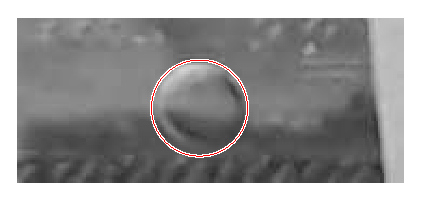
\includegraphics[width=\textwidth]{Figures/SizeFinder/SizeFinder6.eps}
                        \caption{Detected Circle}
                        \label{fig:size:6}
                    \end{subfigure}
                    \caption{Figure }\label{fig:size}
                \end{figure}
            
            There are a few drawbacks to this algorithm. For one, it is highly sensitive to noise, meaning that if the oil is cloudy then it will fail. The top-hat filter is also semi-manual, and must be tweaked for different droplet colours/transparencies. It also struggles with droplets with a radius below 0.3 mm. Finally, it also relies on our assumption that the droplets are perfectly spherical, which is not completely true.\\
            
            The error produced by this algorithm was also considered. As we will discuss later, determination of droplet radius only requires knowledge of the width of a bounding box drawn around the sphere. As such, the diameter of 20 droplets of approximately fixed size was determined both by hand and by algorithm to the nearest pixel. 100\% of the droplets were detected by the algorithm to within 4 pixels in diameter. Given that the diameter of the 2mm thick channel corresponded to approximately 80 pixels, it can be estimated that the boundary of a droplet can be calculated to within 5\% error. \\
            
            This error is largely due to the pixel-level precision and small number of pixels taken up by the droplet. As the droplets produced for the experiment were typically 25 pixels in radius, they only took up 2000 of the 2073600 pixels in a 1920 x 1080 image. If the camera had a lower focal length it could be positioned far closer to the droplet, allowing droplets to take up more than 0.1\% of the pixels of the image. A higher resolution camera would also increase the accuracy of boundary detection. \\
            
            With knowledge of the perimeter of the droplet, a bounding box could be placed around each droplet, pixels converted to mm, and Equation \ref{eq:radii} used to determine the droplet radius.
            
            From this point, the motor could be re-engaged, and the photodiode probed.
    
    \subsection{Oscillating Droplets}
        
        We attempted to oscillate droplets using a variety of methods. Using the control circuitry shown in Figure \ref{fig:MotorCircuit}, the motor could be driven
        
    \subsection{Laser \& Photodiode}
    
        Because oscillations were could be expected to occur at frequencies higher than the 30 Hz (i.e. 30 FPS) the webcam could capture at, a photodiode circuit was created to capture oscillations. (Couldn't get camera close enough?) Because droplets could be assumed to have a different refractive index to that of the carrier oil\cite{viscosity1,viscosity2}, it followed that the presence of a droplet would cause laser light to be scattered differently. Further, as the shape of droplets would vary as the oscillated, they would cause light to scatter in proportion to their degree of oscillation. To observe this effect, a laser was set up as shown in Figure \ref{fig:control}, with the laser on one side of the slide and a photodiode on the other. Because droplets would be moving as they oscillated, the laser was focused on a wide area of the slide. However, because the laser was brightest about its focal point, the system would be more sensitive around this region than others. To improve the region of sensitivity, the solid angle of this bright region was increased by setting the laser up at a glancing angle of over 45$^{\circ}$ to the slide, instead of face on.\\
        
        To amplify the output of the photodiode, a simple circuit was set up\cite{artofelectronics}. The variable resistor was used to act as a gain control, allowing the output voltage to be made as high as possible within the recording range of the DAQ card. The 200 pF capacitor was not originally included, but was later added to reduce noise. A larger capacitor reduces more noise, but makes the circuit less sensitive to small changes (i.e. oscillations).
    
        \begin{figure}[H]
            \centering
            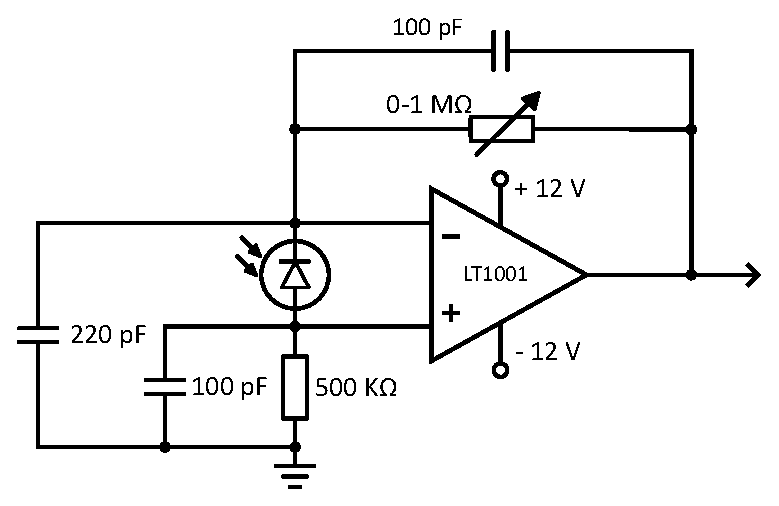
\includegraphics[scale=0.8]{Figures/PDCircuit.eps}
            \caption{Caption}
            \label{fig:my_label}
     \end{figure}
    
    
    
    \subsection{Running Experiments}
        Through creation of a user-friendly toolbox, experimenting could be done automatically with minimimum setup.
        
        \begin{figure}
            \centering
            \hspace*{-5.4cm}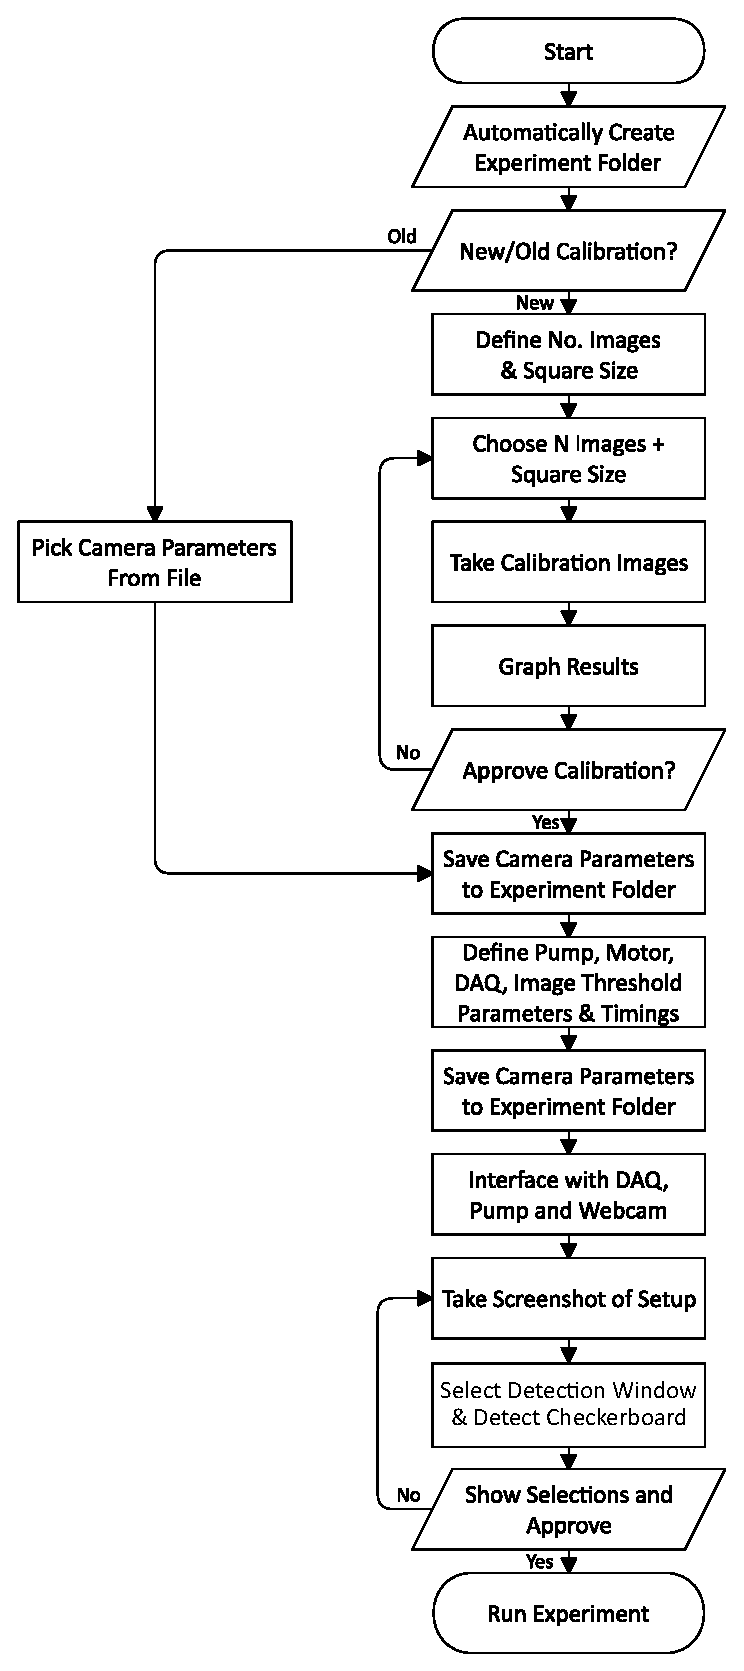
\includegraphics[scale=0.8]{Figures/FlowSetup.eps}
            \caption{Caption}
            \label{fig:setup:flow}
        \end{figure}
        
        \begin{figure}
            \centering
            \hspace*{-1cm}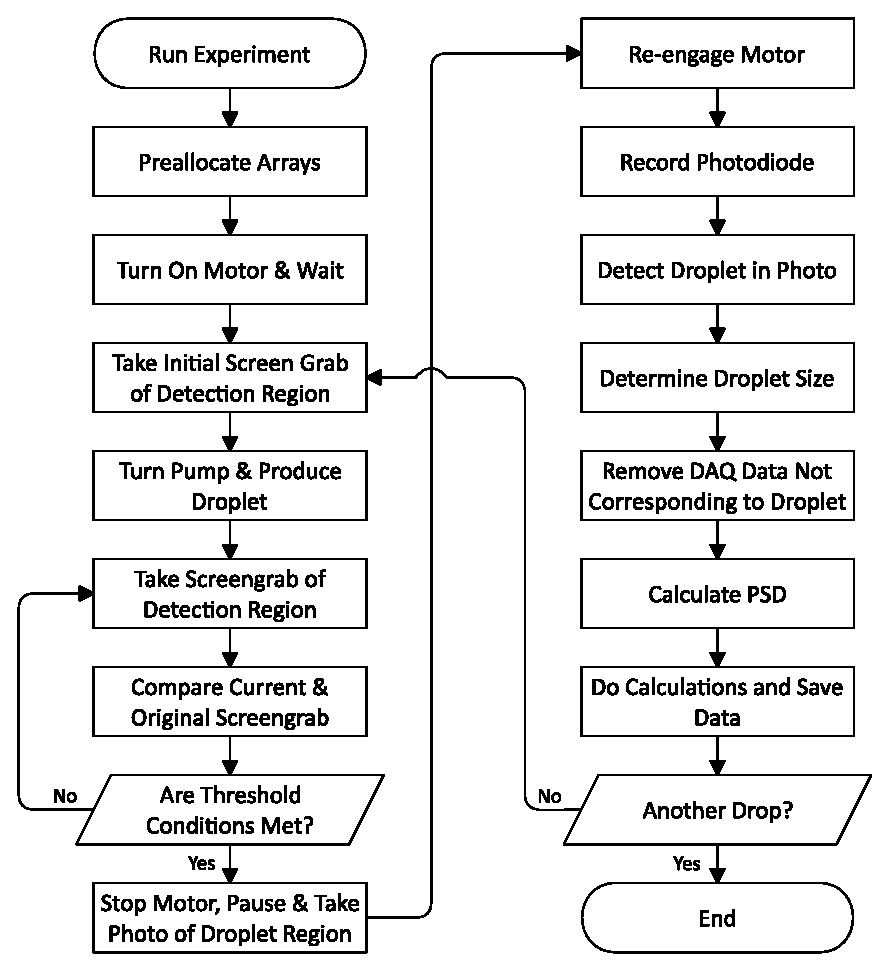
\includegraphics[scale=0.8]{Figures/FlowLogic.eps}
            \caption{Caption}
            \label{fig:setup:logic}
        \end{figure}
    
\section{Results}
    
    \subsection{Motor}
    
        The motor agrees with its rated values (cite).
    
    \subsection{Calibration}
     As shown in Figure \ref{fig:calib:error}, the extrinsics of the camera were calculated to a sub-pixel accuracy of 0.41 pixels, indicating a high quality calibration which will produce errors of less than the precision of the droplet finding algorithm discussed later. Across the 20 calibration images, there was a mean error of X, with all images being calibrated to a standard deviation of Y. This indicates...\\
        
    
    It was found that a 10x11, 0.20mm checkerboard gave the lowest error of 0.03mm. This is shown in Figure \ref{fig:calibsize}. 
        
            \begin{figure}[H]
                \centering
                \hspace*{-1cm}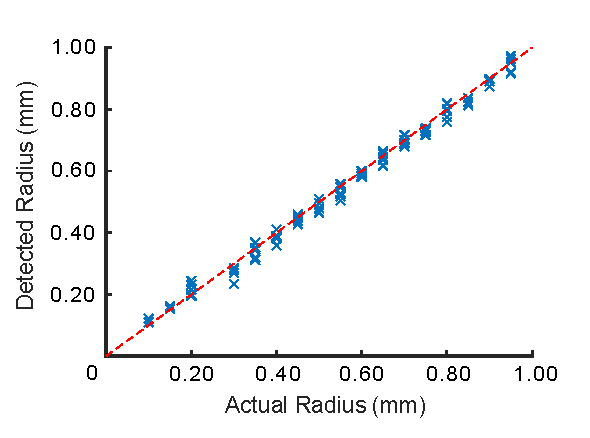
\includegraphics{Figures/CameraCalib.eps}
                \caption{Caption}
                \label{fig:calibsize}
            \end{figure}
        
        From here, it can clearly be seen that the algorithm works as intended (more words)

    \subsection{Oscillating Droplets}
        \subsubsection{Motor Control}
        \subsubsection{Electric Field}
        \subsubsection{Distortion}
    
\section{Discussion}

was written to automatically interface with the pump over a COM port. This also has a significant delay, reducing the throughput of droplets.\\

As we assume that the droplet remains at constant volume, only liquids can be explored as they are incompressible.
% -----------
% REFERENCES
% -----------
\newpage

\bibliographystyle{unsrtnat}
\bibliography{references}
    

% -----------
% FIN
% -----------
\end{document}